%  A simple AAU report template.
%  2015-05-08 v. 1.2.0
%  Copyright 2010-2015 by Jesper Kjær Nielsen <jkn@es.aau.dk>
%
%  This is free software: you can redistribute it and/or modify
%  it under the terms of the GNU General Public License as published by
%  the Free Software Foundation, either version 3 of the License, or
%  (at your option) any later version.
%
%  This is distributed in the hope that it will be useful,
%  but WITHOUT ANY WARRANTY; without even the implied warranty of
%  MERCHANTABILITY or FITNESS FOR A PARTICULAR PURPOSE.  See the
%  GNU General Public License for more details.
%
%  You can find the GNU General Public License at <http://www.gnu.org/licenses/>.
%
%  A simple AAU report template.
%  2015-05-08 v. 1.2.0
%  Copyright 2010-2015 by Jesper Kjær Nielsen <jkn@es.aau.dk>
%
%  This is free software: you can redistribute it and/or modify
%  it under the terms of the GNU General Public License as published by
%  the Free Software Foundation, either version 3 of the License, or
%  (at your option) any later version.
%
%  This is distributed in the hope that it will be useful,
%  but WITHOUT ANY WARRANTY; without even the implied warranty of
%  MERCHANTABILITY or FITNESS FOR A PARTICULAR PURPOSE.  See the
%  GNU General Public License for more details.
%
%  You can find the GNU General Public License at <http://www.gnu.org/licenses/>.
%
\documentclass[11pt,twoside,a4paper,openright]{report}
%%%%%%%%%%%%%%%%%%%%%%%%%%%%%%%%%%%%%%%%%%%%%%%%
% Language, Encoding and Fonts
% http://en.wikibooks.org/wiki/LaTeX/Internationalization
%%%%%%%%%%%%%%%%%%%%%%%%%%%%%%%%%%%%%%%%%%%%%%%%
% Select encoding of your inputs. Depends on
% your operating system and its default input
% encoding. Typically, you should use
%   Linux  : utf8 (most modern Linux distributions)
%            latin1 
%   Windows: ansinew
%            latin1 (works in most cases)
%   Mac    : applemac
% Notice that you can manually change the input
% encoding of your files by selecting "save as"
% an select the desired input encoding. 
\usepackage[utf8]{inputenc}			% Character encoding
%\usepackage[utf8]{inputenc}
% Make latex understand and use the typographic
% rules of the language used in the document.
\usepackage[danish]{babel}

\usepackage{tabu}
\usepackage{array}
\newcolumntype{?}{!{\vrule width 1.1pt}}
\usepackage{makecell}
% Use the palatino font
\usepackage[sc]{mathpazo}
\newcommand{\thickhline}{\Xhline{1.1pt}}
\linespread{1.05}         % Palatino needs more leading (space between lines)
% Choose the font encoding
%\usepackage[T1]{fontenc}
%%%%%%%%%%%%%%%%%%%%%%%%%%%%%%%%%%%%%%%%%%%%%%%%
% Graphics and Tables
% http://en.wikibooks.org/wiki/LaTeX/Importing_Graphics
% http://en.wikibooks.org/wiki/LaTeX/Tables
% http://en.wikibooks.org/wiki/LaTeX/Colors
%%%%%%%%%%%%%%%%%%%%%%%%%%%%%%%%%%%%%%%%%%%%%%%%
% load a colour package
\usepackage{xcolor}
\definecolor{aaublue}{RGB}{33,26,82}% dark blue
% The standard graphics inclusion package
\usepackage{graphicx}
\graphicspath{{./grafik/}}
\usepackage{rotating}
% Set up how figure and table captions are displayed
\usepackage{caption}
\captionsetup{%
  font=footnotesize,% set font size to footnotesize
  labelfont=bf % bold label (e.g., Figure 3.2) font
}
\usepackage{pdfpages}
\usepackage[natbib=true, style=numeric, backend=bibtex, sorting=none,maxbibnames=99]{biblatex}
\DefineBibliographyStrings{danish}{andothers = {et\addabbrvspace al\adddot}}
\setcounter{biburlucpenalty}{8000}
\setcounter{biburllcpenalty}{7000}
% Make the standard latex tables look so much better
\usepackage{array,booktabs}
% Enable the use of frames around, e.g., theorems
% The framed package is used in the example environment
\usepackage{framed}
\usepackage[linewidth=2pt]{mdframed} %Bliver brugt til at lave en ramme om ting

%%%%%%%%%%%%%%%%%%%%%%%%%%%%%%%%%%%%%%%%%%%%%%%%
% Mathematics
% http://en.wikibooks.org/wiki/LaTeX/Mathematics
%%%%%%%%%%%%%%%%%%%%%%%%%%%%%%%%%%%%%%%%%%%%%%%%
% Defines new environments such as equation,
% align and split 
\usepackage{amsmath}
% Adds new math symbols
\usepackage{amssymb}
% Use theorems in your document
% The ntheorem package is also used for the example environment
% When using thmmarks, amsmath must be an option as well. Otherwise \eqref doesn't work anymore.
\usepackage[framed,amsmath,thmmarks]{ntheorem}

%%%%%%%%%%%%%%%%%%%%%%%%%%%%%%%%%%%%%%%%%%%%%%%%
% Page Layout
% http://en.wikibooks.org/wiki/LaTeX/Page_Layout
%%%%%%%%%%%%%%%%%%%%%%%%%%%%%%%%%%%%%%%%%%%%%%%%
% Change margins, papersize, etc of the document
\usepackage[
  inner=28mm,% left margin on an odd page
  outer=41mm,% right margin on an odd page
  ]{geometry}
% Modify how \chapter, \section, etc. look
% The titlesec package is very configureable
\usepackage{titlesec}
\titleformat{\chapter}[display]{\normalfont\huge\bfseries}{\chaptertitlename\ \thechapter}{20pt}{\Huge}
\titleformat*{\section}{\normalfont\Large\bfseries}
\titleformat*{\subsection}{\normalfont\large\bfseries}
\titleformat*{\subsubsection}{\normalfont\normalsize\bfseries}
%\titleformat*{\paragraph}{\normalfont\normalsize\bfseries}
%\titleformat*{\subparagraph}{\normalfont\normalsize\bfseries}

% Clear empty pages between chapters
\let\origdoublepage\cleardoublepage
\newcommand{\clearemptydoublepage}{%
  \clearpage
  {\pagestyle{empty}\origdoublepage}%
}
\let\cleardoublepage\clearemptydoublepage

% Change the headers and footers
\usepackage{fancyhdr}
\pagestyle{fancy}
\fancyhf{} %delete everything
\renewcommand{\headrulewidth}{0pt} %remove the horizontal line in the header
\fancyhead[RE]{\small\nouppercase\leftmark} %even page - chapter title
\fancyhead[LO]{\small\nouppercase\rightmark} %uneven page - section title
\fancyhead[LE,RO]{\thepage} %page number on all pages
% Do not stretch the content of a page. Instead,
% insert white space at the bottom of the page
\raggedbottom
% Enable arithmetics with length. Useful when
% typesetting the layout.
\usepackage{calc}

%%%%%%%%%%%%%%%%%%%%%%%%%%%%%%%%%%%%%%%%%%%%%%%%
% Bibliography
% http://en.wikibooks.org/wiki/LaTeX/Bibliography_Management
%%%%%%%%%%%%%%%%%%%%%%%%%%%%%%%%%%%%%%%%%%%%%%%%
%\usepackage[backend=bibtex,
%  bibencoding=utf8
%  ]{biblatex}
%\addbibresource{bib}

%%%%%%%%%%%%%%%%%%%%%%%%%%%%%%%%%%%%%%%%%%%%%%%%
% Misc
%%%%%%%%%%%%%%%%%%%%%%%%%%%%%%%%%%%%%%%%%%%%%%%%
% Add bibliography and index to the table of
% contents
\usepackage[nottoc]{tocbibind}
% Add the command \pageref{LastPage} which refers to the
% page number of the last page
\usepackage{lastpage}
% Add todo notes in the margin of the document
\usepackage[
%  disable, %turn off todonotes
  colorinlistoftodos, %enable a coloured square in the list of todos
  textwidth=\marginparwidth, %set the width of the todonotes
  textsize=scriptsize, %size of the text in the todonotes
  ]{todonotes}

%%%%%%%%%%%%%%%%%%%%%%%%%%%%%%%%%%%%%%%%%%%%%%%%
% Hyperlinks
% http://en.wikibooks.org/wiki/LaTeX/Hyperlinks
%%%%%%%%%%%%%%%%%%%%%%%%%%%%%%%%%%%%%%%%%%%%%%%%
% Enable hyperlinks and insert info into the pdf
% file. Hypperref should be loaded as one of the 
% last packages
\usepackage{hyperref}
\hypersetup{%
	pdfpagelabels=true,%
	plainpages=false,%
	pdfauthor={Author(s)},%
	pdftitle={Title},%
	pdfsubject={Subject},%
	bookmarksnumbered=true,%
	colorlinks=true,%
	citecolor=black,%
	filecolor=black,%
	linkcolor=black,% you should probably change this to black before printing
	urlcolor=black,%
	pdfstartview=FitH%
}

\usepackage{enumitem}
\usepackage{caption}
\usepackage{subcaption}
\usepackage[danish,nameinlink,capitalise]{cleveref}
\usepackage{listings}
\usepackage{verbatim} % For the comment environment, that allows for commenting out large blocks.

% Additional commands
\newcommand{\namedtodo}[5]
{
  \ifthenelse{\equal{#1}{}}
  {
    \todo[backgroundcolor=#4,caption=
    {\textbf{#3: } #2}
    ,inline]
    {\color{#5}\textbf{#3: }#2}
  }
  {
    \todo[backgroundcolor=#4,caption=
    {\textbf{#3: } #1}
    ,inline]
    {\color{#5}\textbf{#3: }#2}
  }
}
\newcommand{\mikkel}[2][]{\namedtodo{#1}{#2}{Mikkel}{blue!80}{white}}
\newcommand{\stefan}[2][]{\namedtodo{#1}{#2}{Stefan M}{orange}{black}}
\newcommand{\mikael}[2][]{\namedtodo{#1}{#2}{Mikael}{green}{black}}
\newcommand{\bruno}[2][]{\namedtodo{#1}{#2}{Bruno}{black!10!red!90}{white}}
\newcommand{\lasse}[2][]{\namedtodo{#1}{#2}{Lasse}{black!10!yellow!90}{black}}
\newcommand{\als}[2][]{\namedtodo{#1}{#2}{Als}{purple!90!orange}{white}}
\newcommand{\winde}[2][]{\namedtodo{#1}{#2}{Winde}{black}{white}}
\newcommand{\lars}[2][]{\namedtodo{#1}{#2}{Lars}{blue!80}{black}}
\newcommand{\ivan}[2][]{\namedtodo{#1}{#2}{Ivan}{red}{black}}


  \makeatletter \renewcommand \listoftodos{\section*{List of Todos} \@starttoc{tdo}}
  \renewcommand\l@todo[2]
    {\par\noindent \textit{#2}, \parbox{10cm}{#1}\par} \makeatother
% Her er en liste over navnene på de forskellige styles
% C#: csharp
% F#: fsharp

% 
% Listings kan refereres vha. \cref{}
\crefname{listing}{code example}{code example}
\Crefname{listing}{Code example}{code examples}
% 

%Algoritmer i cref
\crefname{algocf}{algorithm}{algorithm}
\Crefname{algocf}{Algorithm}{Algorithms}
%Algoritmelinjer i cref
\crefalias{AlgoLine}{line}%

\makeatletter
\let\cref@old@stepcounter\stepcounter
\def\stepcounter#1{%
  \cref@old@stepcounter{#1}%
  \cref@constructprefix{#1}{\cref@result}%
  \@ifundefined{cref@#1@alias}%
    {\def\@tempa{#1}}%
    {\def\@tempa{\csname cref@#1@alias\endcsname}}%
  \protected@edef\cref@currentlabel{%
    [\@tempa][\arabic{#1}][\cref@result]%
    \csname p@#1\endcsname\csname the#1\endcsname}}
\makeatother
%

% Angivelse af navn på listings
\renewcommand\lstlistingname{Code example}
\renewcommand\lstlistlistingname{Code example}

\lstdefinestyle{standard}
{
	frame=shadowbox,
	framesep=5pt,
	rulecolor=\color{blue!40!black},
	rulesepcolor=\color{white!93!black},
	numbers=left,
	basicstyle=\ttfamily,
	numberstyle=\tiny,
	numberfirstline=true,
	%numberblanklines=false,
	stepnumber=1,
	numbersep=9pt,	
	captionpos=b,
	escapeinside={(*}{*)},
	breaklines=true,
	tabsize=4,
	language=c
}

\lstset{style=standard}

\lstdefinestyle{c}
{
	style=standard
}

\lstdefinestyle{csmall}
{
	style=c
}

\lstdefinestyle{csharp}
{
	style=standard,
	language=[Sharp]C
}
\lstdefinestyle{csharpsmall}
{
	style=csharp
}
\lstdefinestyle{fsharp}
{
	language=[Sharp]F,
	frame=lr,
	rulecolor=\color{blue!80!black}
}
\lstdefinestyle{fsharpsmall}
{
	style=fsharp,
	basicstyle=\ttfamily\footnotesize
}


% Definitions

% Superscript and subscript
\newcommand{\superscript}[1]{\ensuremath{^{\textrm{#1}}}}
\newcommand{\subscript}[1]{\ensuremath{_{\textrm{#1}}}}

% Degrees
\newcommand{\degree}{\ensuremath{^\circ}}
\newcommand{\dg}{\degree}

\newcommand{\quoter}[1]%
{
  \par
  \vspace{1.5em}
  \addtolength{\leftskip}{1.5cm}
  \addtolength{\rightskip}{1.5cm}
  \textit{#1}
  \addtolength{\leftskip}{-1.5cm}
  \addtolength{\rightskip}{-1.5cm}
  \vspace{1.5em}
  \par
}


\newcommand{\sensor}[3]
{
	\section{#1}
	#2
	
	#3
}

\newcommand{\analyse}[2]
{
\subsection{#1}
#2
}


% package inclusion and set up of the document
% see, e.g., http://en.wikibooks.org/wiki/LaTeX/Formatting#Hyphenation
% for more information on word hyphenation
\hyphenation{ex-am-ple hy-phen-a-tion short}
\hyphenation{long la-tex}
% 
%  A simple AAU report template.
%  2015-05-08 v. 1.2.0
%  Copyright 2010-2015 by Jesper Kjær Nielsen <jkn@es.aau.dk>
%
%  This is free software: you can redistribute it and/or modify
%  it under the terms of the GNU General Public License as published by
%  the Free Software Foundation, either version 3 of the License, or
%  (at your option) any later version.
%
%  This is distributed in the hope that it will be useful,
%  but WITHOUT ANY WARRANTY; without even the implied warranty of
%  MERCHANTABILITY or FITNESS FOR A PARTICULAR PURPOSE.  See the
%  GNU General Public License for more details.
%
%  You can find the GNU General Public License at <http://www.gnu.org/licenses/>.
%
%
%
% see, e.g., http://en.wikibooks.org/wiki/LaTeX/Customizing_LaTeX#New_commands
% for more information on how to create macros

%%%%%%%%%%%%%%%%%%%%%%%%%%%%%%%%%%%%%%%%%%%%%%%%
% Macros for the titlepage
%%%%%%%%%%%%%%%%%%%%%%%%%%%%%%%%%%%%%%%%%%%%%%%%
%Creates the aau titlepage
\setlength{\fboxsep}{10pt} % Use this to change margins of abstract.
\newcommand{\aautitlepage}[3]{%
  {
    %set up various length
    \ifx\titlepageleftcolumnwidth\undefined
      \newlength{\titlepageleftcolumnwidth}
      \newlength{\titlepagerightcolumnwidth}
    \fi
    \setlength{\titlepageleftcolumnwidth}{0.5\textwidth-\tabcolsep}
    \setlength{\titlepagerightcolumnwidth}{\textwidth-2\tabcolsep-\titlepageleftcolumnwidth}
    %create title page
    \thispagestyle{empty}
    \noindent%
    \begin{tabular}{@{}ll@{}}
      \parbox{\titlepageleftcolumnwidth}{
        \iflanguage{danish}{%
          
\includegraphics[width=.8\titlepageleftcolumnwidth]{aau_logo_da}
        }{%
          
\includegraphics[width=.8\titlepageleftcolumnwidth]{aau_logo_en}
        }
      } &
      \parbox{\titlepagerightcolumnwidth}{\raggedleft\sf\small
        #2
      }\bigskip\\
       #1 &
      \parbox[t]{\titlepagerightcolumnwidth}{%
      \textbf{Abstract:}\bigskip\par
        \fbox{\parbox{\titlepagerightcolumnwidth-2\fboxsep-2\fboxrule}{%
          #3
        }}
      }\\
    \end{tabular}
    \vfill
    \iflanguage{danish}{%
      \noindent{\footnotesize\emph{Rapportens indhold er frit tilgængeligt, men offentliggørelse (med kildeangivelse) må kun ske efter aftale med forfatterne.}}
    }{%
      \noindent{\footnotesize\emph{The content of this report is freely available, but publication (with reference) may only be pursued due to agreement with the author.}}
    }
    \clearpage
  }
}

%Create english project info
\newcommand{\englishprojectinfo}[8]{%
  \parbox[t]{\titlepageleftcolumnwidth}{
    \textbf{Title:}\\ #1\bigskip\par
    \textbf{Theme:}\\ #2\bigskip\par
    \textbf{Project Period:}\\ #3\bigskip\par
    \textbf{Project Group:}\\ #4\bigskip\par
    \textbf{Participant(s):}\\ #5\bigskip\par
    \textbf{Supervisor(s):}\\ #6\bigskip\par
    \textbf{Copies:} #7\bigskip\par
    \textbf{Page Numbers:} \pageref{LastPage}\bigskip\par
    \textbf{Date of Completion:}\\ #8
  }
}

%Create danish project info
\newcommand{\danishprojectinfo}[8]{%
  \parbox[t]{\titlepageleftcolumnwidth}{
    \textbf{Titel:}\\ #1\medskip \par
    \textbf{Tema:}\\ #2\medskip \par
    \textbf{Projektperiode:}\\ #3\medskip \par
    \textbf{Projektgruppe:}\\ #4\medskip \par
    \textbf{Deltagere:}\\ #5\medskip \par
    \textbf{Vejleder:}\\ #6\medskip \par
    \textbf{Oplagstal:} #7\medskip \par
    \textbf{Sidetal:} \pageref{LastPage}\medskip \par
    \textbf{Afleveringsdato:}\\ #8
  }
}

%%%%%%%%%%%%%%%%%%%%%%%%%%%%%%%%%%%%%%%%%%%%%%%%
% An example environment
%%%%%%%%%%%%%%%%%%%%%%%%%%%%%%%%%%%%%%%%%%%%%%%%
\theoremheaderfont{\normalfont\bfseries}
\theorembodyfont{\normalfont}
\theoremstyle{break}
\def\theoremframecommand{{\color{gray!50}\vrule width 5pt \hspace{5pt}}}
\newshadedtheorem{exa}{Example}[chapter]
\newenvironment{example}[1]{%
		\begin{exa}[#1]
}{%
		\end{exa}
}
% my new macros


\begin{document}
%frontmatter
\pagestyle{empty} %disable headers and footers
\pagenumbering{roman} %use roman page numbering in the frontmatter
%\hspace*{-1cm}\parbox[b][\textheight][t]{\textwidth}
{

\begin{center}
	
\includegraphics[height=5.2cm]{aau_logo_da}\\
	\vspace{0.25cm}
	%Student Report
\end{center} 

\vspace{1cm}
\begin{center}

\textbf{\Huge {Software 8 - PsyLog: Søvn og Aktivitetsmoduler for Personer med Psykiske Lidelser}} \\ \vspace{0.5cm}
%\textbf{\Large {Developing Complex Software Systems:}} \\ \vspace{.5cm}
%\textbf{\huge {GIRAF Web Admin and GIRAF Timer}} \\ \vspace{1cm}
\textbf{\Large P8 Projekt af SW808F15}\\ \vspace{0.5cm}
\textbf{\large 2. februar 2015 til 27. maj 2015}\\
\end{center}



\vspace{0.25cm}
\begin{center}
\item {\textbf{Deltagere:}} \\
Søren Skibsted Als\\
Lars Andersen\\
Lasse Vang Gravesen\\
Mathias Winde Pedersen
\end{center}

\thispagestyle{empty}

\newpage
\thispagestyle{empty}
\mbox{}
}
%\input{sections/colophon.tex}
\pdfbookmark[0]{Titelblad}{label:titlepage_da}
\aautitlepage{%
  \danishprojectinfo{
    Rapportens titel %title
  }{%
    Semestertema %theme
  }{%
    Forårssemestret 2015 %project period
  }{%
    SW808 % project group
  }{%
    %list of group members
    \textbf{SW808:}\\
    Lars Andersen\\
    Lasse Vang Gravesen\\
    Mathias Winde Pedersen\\
    Søren Skibsted Als
  }{%
    %list of supervisors
    Ivan Aaen
  }{%
    1 % number of printed copies
  }{%
    \today % date of completion
  }%
}{%department and address
  \textbf{Elektronik og IT}\\
  Aalborg Universitet\\
  \href{http://www.aau.dk}{http://www.aau.dk}
}{}

\cleardoublepage

%\section*{Forord}
%Denne rapport blev lavet ved Aalborg Universitet i andet semester af Software kandidat studiet af gruppen sw808f15.
Projektet var et del projekt af PsyLog projektet \citep{misc:faellesrapp}, som blev udviklet i samarbejde med sw807f15.
Rapporten er lavet som en del af P8 projektet mellem d. 2. februar 2015 og d. 27. maj 2015.
Projektet blev vejledt af Ivan Aaen, hvis vejledning var meget værdsat.
Derudover er projektet foreslået af Morten Aagaard som gennem projektet agerede som binde-
led mellem projektgruppen og specialister indenfor psykologi. Dette resulterede
blandt andet i møder med psykolog Janne Vedel Rasmussen, psykiater Jørgen Aa-
gaard, og et fokusgruppe interview med patienter med affektive lidelser. Hans
hjælp, råd samt indsigt i faget var en stor hjælp for projektet.
Derudover skal der også lyde en stor tak til patienterne, psykolog Janne Vedel Rasmussen og psykiater Jøren Aagaard for deres deltagelse.
\als{Lige nu er det samme tekst der er kopieret ind her, måske skal man omformulere... dunno kan også være det ikke er nødvendigt}
%\cleardoublepage

\pdfbookmark[0]{Indholdsfortegnelse}{label:contents}
\pagestyle{fancy} %enable headers and footers again
\setcounter{tocdepth}{1}
\tableofcontents
\listoftodos
%\input{sections/preface.tex}
\cleardoublepage
%mainmatter
\pagenumbering{arabic} %use arabic page numbering in the mainmatter

\chapter{Introduktion}
Idag er der mange danskere som lider af psykiske lidelser hvilket tydeligt kan ses fra bruget af antidepressiv medicin idet at 1 af 12 danskere i 2011 brugte det \citep{misc:forbrugAntidepressiva}. 

Disse personer har selvfølgelig helbreds veje til at komme under behandling, så som terapi behandling eller medicinsk behandling.
Men som patienter ved et fokusgruppe møde sagde, REF, ville ethvert værktøj som kan gøre deres liv nemmere eller bedre være godt.
Der er mange åbne veje for innovation i dette område, men noget af det mest relevante og interessante er at se på hvordan man kan bruge smartphones til at hjælpe disse personer.
Dette er klart da næsten 80\% af danskere har adgang til smartphones \citep{misc:dstElektronik}, og disse smartphones er et kraftfuldt værktøj som kan bruges på mange forskellige måder og mange af disse uudforskede.

Dette ligger som baggrund for den modulære fælles platform(eller `PsyLog'), REF TIL FÆLLES RAPPORT, hvor et mobilt system til indsamling af sensor og brugs data er blevet gjort mulig samt en platform som gør det muligt at lave udregninger og visninger af disse.

Ved mange psykiske lidelser ser man tit at der er opførsels mønstre som signalerer selve sygdommen, idet at visse sygdomme har symptomer som materaliserer sig som ændring i opførsel.
Et eksempel på dette kunne f.eks. hvad man ser med scizofrene som har nedsat social interaktion \citep{misc:negativeSymptomsSchizo}. 

I kombination med den fælles platform og faktaen at sygdomme har symptomer som materaliserer sig som ændring i opførsel og at dette muligvis kan opdages tidligt gennem brug af sensor data og derved bruges til at informere brugeren. 

Vores fokus er som allerede sagt i fælles rapporten på personer med unipolar og bipolar depression. 
For personer med disse lidelser er der forskellige indikatorer, som f.eks. nedsat fysisk aktivitet og social aktivitet, søvn problemer, indre uro, dårlig appetit, humør, man skal tvinge sig selv til at gøre alting og så videre. % ref til fokusgruppe møde
Af disse kan fysisk og social aktivitets niveau søvn måles ved hjælp af data som kan optages fra en smartphone. 
Her vælger vi at fokusere primært på søvn da det gentagne gange er blevet sagt fra psyloger, psykiatere og patienter(ref til det de sagde) at søvn problemer er et af de mest sete symptomer når det kommer til personer med unipolar og bipolar depression, på samme tid vil det også blive forsøgt at måle på fysisk aktivitets niveau da det kan simplificeres og måles meget let.

På baggrund af dette giver det mening at udvikle moduler som kan hjælpe disse personer idet at hvis de kan se hvor meget de sover eller hvor aktive de er giver det dem et overblik og dette vil så hjælpe dem med at tage beslutninger om hvad de skal gøre. 
Dette vil inkludere udvikling af moduler som enten gemmer ny data fra en sensor eller analyserer eksisterende data.

\chapter{Analyse}
\section{Søvn Analyse}
Forskning viser at søvn har en væsentlig indflydelse på ens tilstand, dette gælder i høj grad bipolare patienter \citep{CPSP:CPSP1164}.
Vi har også hørt gentagne gange fra psykologer, psykiatere og patienter at det er et meget fremtædent symptom for både unipolar og bipolar depression. REF.

Det viser sig at en regelmæssig søvn-vågen cykel er særdeles vigtig for bipolare patienter.
Eksempelvis kan mangel på søvn medføre større risiko for at gå ind i en mani- eller depressions-periode \citep{CPSP:CPSP1164}.

Derudover er ændring i søvnmængde et tydeligt tegn på en mani- eller depressions-periode, jævnfør tidligere sektion REFERER TIL DEN.
Hvis man er i en maniperiode sover man væsentligt mindre end for den habituelle periode \citep{CPSP:CPSP1164}.
Modsat for depression vil man typisk sove væsentligt længere end for den habituelle periode, men vi har også hørt fra patienter at de også kan have problemer med at sove.

Grundet dette anses søvn for en vigtig indikator på om man begynder at befinde sig i en mani- eller depressions-periode og bør derfor undersøges nærmere til at determinere sådanne perioder.

\section{Søvn Estimerings Metoder}
Da søvn er en meget vigtig faktor til estimering af sygdomme og livskvalitet er der lagt en stor mængde forskning i dette område.
Dette giver udslag i en lang række af søvnestimeringsmetoder, hvor nogle af de mest fremtrædende muligheder nævnes og vurderes i forhold til fokus for dette projekt.

\subsection{Polysomnografi}
Den måske mest akkurate søvnestimerings metode er polysomnografi, der er en metode der kombinerer et elektroencefalogram med målinger af muskel spænding og øjenbevægelse \citep{misc:polysomnografi,misc:polysomnography}.
Dog kræver denne metode en større mængde af special udstyr og erfarne teknikere til at montere udstyret på en patient, hvilket gør denne metode upraktisk i en almen patients soveværelse.

\subsection{AktiGrafi}
Imidlertid findes der andre metoder der er nemmere at benytte.
Et eksempel på sådan en søvnestimerings metode er aktigrafi, der er akkurat selvom det kun benytter sig af accelerometre påmonteret ens arm.
En sådan teknik kan estimere metrikker såsom timer sovet, søvn virkningsgrad, og antal af søvnafbrydelser.
Kendte eksempler på sådanne apparater findes ved eksempelvis FitBit og JawBone \citep{misc:fitbitSleepTracking,misc:jawBoneSleepTracking}.
Prisen på disse kan svinge fra 500 kroner til 2000 kroner baseret på hvilket produkt man køber, og påkræver at armbåndet er påmonteret når man sover.

Kravet om at udstyr som FitBit og JawBone skal være monteret på ens arm finder vi ikke som en tilstrækkelig hæmning for at afvise brugen af sådan en teknik.
Af samme grund står muligheden åben for at bruge sådant udstyr i fremtiden, hvis man er interesseret i mere akkurat søvn estimering end efterfølgende nævnte estimerings metoder.
Derudover er platformen opbygget til at være yderst fleksibelt angående hvilke moduler kan benyttes, så skulle man i fremtiden ønske at udvikle et modul der virker med FitBit/JawBone er dette muligt, men udskydes på pågældende tidspunkt grundet ressourcemangel i form af arbejdstid og det fornødne udstyr tilrådigt.
Der findes lignende løsninger der kun benytter sig af ens smartphone, men hvor man pålægger patienten at placere sin smartphone under hovedpuden.
Men ligesom FitBit/JawBone løsningen kræver det at man overdrager ansvaret til patienten om at placere smartphonen i sengen, ligesom med armbåndene skal monteres på ens arm.

\subsection{Søvn Dagbog}
Der findes en lang række spørgeskemaer, hvor patienten får ansvaret for at udfylde sådanne skemaer, hvor man på den måde kan følge en patients søvnrytme.
Sådanne metoder er ikke vores fokus emne, men er en mulighed med den fleksible platform der er udviklet, hvor en sådan dagbog er et modul.
Dog er det værd at tage med i betragtning, når man skal lære en ny model, hvilket \cite{Min:2014:TNT:2556288.2557220} angiver, hvor man bruger dagbogen som "ground truth" til at træne ens model.

Med ressourcerne for dette projekt er dette dog ikke valgt som primær fokus, da vi ønsker en metode der kan estimere søvn med mindst mulig bruger intervention, og hvor grundlaget for vurdering skal være ved hjælp af sensorer fremfor en subjektiv vurdering man alligevel har mulighed for i forvejen.
Idéen om en "objektiv dagbog" er dermed også i tankerne her, og er hvorfor denne løsning ikke undersøges nærmere end at det kan bruges for læringsperioder for vores modeller.

\subsection{Toss 'N' Turn}
Følgende fremgangsmåde er præsenteret i \cite{Min:2014:TNT:2556288.2557220}, og beskrivelsen bygger på forskningsresultaterne præsenteret deri.

For Toss 'N' Turn fremgangsmåden er tanken at man blot skal have sin smartphone lokaliseret i sit soveværelse for at den kan estimere ens søvnstarttidspunkt, vækketidspunkt og sovelængde.
Teknikken tager udgangspunkt i en række sensorkilder der er tilgængelig på smartphonen i forvejen.
Disse værende accelerometer, mikrofon(maks amplitude), lys sensor, proximity sensor, kørende processer, batteri stadie, og skærmvisningstilstand.
Ud fra disse sensor kilder og en søvndagbog der foretages i minimum tre dage, til at lære en søvnestimeringsmodel, kan de opnå en præcision med søvnlængde ME på under 1 time.
Derudover har deres forskning vist at den gennemsnitlige præcision for daglig søvn estimering er på 83.97 \%. Hvilket gør det til en oplagt mulighed at arbejde med.
Deres algoritme fungere så ved at foretage en række feature udtrækninger, og så bruge teknikker såsom low-pass filter, Naive Bayes classifier og decision trees til at opnå den fornødne nøjagtighed.

En ulempe ved denne teknik er at den kræver en oplæringsperiode på minimum 3 dage for at få en lovende præcision, men er antaget at være et acceptabelt kompromis, da estimeringen så ville kunne fungere relativt præcist efterfølgende.

Derudover er det en klar fordel ved denne teknik at man ikke behøver at placere smartphonen i sengen, og kræver derfor minimal bruger intervention, da mange folk alligevel bruger deres smartphone som vækkeur.

Det ville dog være bedre med en søvnestimeringsteknik der ikke nødvendigvis kræver en træningsperiode.

\subsection{Best Effort Sleep Model}\label{sec:BES}
Best Effort Sleep (BES) Model \citep{6563918} bruger en fremgangsmåde der udelukkende baseres på målbare data fra en smartphone til at estimere en brugers søvnlængde.
Disse målbare datakilder anskaffes på en måde så brugeren ikke behøver ændre sin søvn adfærd, som det fx er tilfældet på andre tilsvarende løsninger som fx JawBone eller FitBit der kræver at en wearable benyttes mens man sover.
Det at ingen af datakilderne er i direkte kontakt med brugeren går dog ud over præcisionen, der er op mod 40 minutters unøjagtighed i estimeringen af søvnlængde.
Om denne unøjagtighed er acceptabel skal vurderes ud fra hvad informationen skal bruges til og hvilke kriterier der er til data.
Ud over dette kan BES ikke bruges til at estimere kvaliteten af ens søvn.
Med kvaliteten menes hvor mange gange man har været vågen i løbet af natten, til dette kræves involvering af brugeren, enten af de bruger en wearable eller at de interagerer med systemet.

I vores tilfælde vil denne fremgangsmåde fungere godt som en backup solution til en af de brugerinvolverende fremgangsmåder, da det største problem ved disse er at de bliver ubrugelige hvis brugeren ikke bruger dem rigtigt.
I de tilfælde hvor BES og en bruger involverende løsning begge er tilstede, kan BES bruges til at validere data fra den brugerinvolverende løsning. 

I BES bruges der seks forskellige målinger til at estimere søvn.
Grunden til det store antal målinger er, at det er nødvendigt med flere forskellige input kilder, da ingen af dem er i direkte kontakt med brugeren og at de hver for sig ikke siger særlig meget men i kombination giver en udmærket estimering om brugeren sover.
\begin{description}[style=nextline]
\item[Lys]
I de fleste tilfælde vurderes det at der er mørkt i det rum hvor man sover. Dog kan der her være visse uregelmæssigheder fx. kan folk der lider af en depression godt leve i mørke hele dagen, og nogle folk kan også godt finde på at sove med lyset tændt. Det er lyset er tændt er dog kun et mindre irritationsmoment.
\item[Lås]
Mens en person sover vil han ikke låse sin telefon op, og den vil normalt låse selv efter en lille periode, dermed ved man også at hvis en telefon bliver låst op, så er personen vågen.
\item[Opladning]
Mange folk sætter deres telefon til opladning mens de sover, derfor kan opladnings perioder give en indikation af søvn, det er dog ikke garanteret at dette er tilfældet.
\item[Slukket]
Nogle folk slukker deres telefon mens de sover for ikke at blive forstyrret, derfor kan man se på længde af disse perioder for at vurdere søvn. Det viste sig dog ud fra test at ingen af testpersonerne gjorde dette. 
\item[Bevægelse]
Når man sover ligger ens telefon sandsynligvis stille, hvorimod bevægelse indikerer man er vågen.
\item[Lyd]
I de fleste tilfælde er det stille når folk sover, bortset fra diverse former for baggrundsstøj, fx snorken, hosten eller lyden af et bilhorn udenfor. Selvom disse er forstyrrende kan de filtreres fra.
\end{description}
 
Disse målinger skal vægtes forskelligt, og ud fra eksperimenterne udført af \citet{6563918}, nåede de frem til følgende vægtning af de forskellige datakilder, se \cref{tab:vaegtninger}.

\begin{table}[h]
\centering
\begin{tabular}{|c|c|}
\hline Datakilde & Koefficient\\
\hline Lys & 0.0415 \\ 
\hline Lås & 0.0512 \\ 
\hline Slukket & 0.0000 \\ 
\hline Opladning & 0.0469 \\ 
\hline Bevægelse & 0.5445 \\ 
\hline Lyd & 0.3484 \\ 
\hline 
\end{tabular}
\caption{De forskellige vægtninger for hver af målingerne.}
\label{tab:vaegtninger}
\end{table}

Disse koefficienter kan bruges af os til at springe en eventuel lærings periode over, dog kan dette gå ud over præcisionen.
Hvis præcisionen var meget vigtig ville man have en lille lærings periode, hvor man får den objektive sandhed om søvnlængden ind, så man kan blive i stand til at finde de optimale koefficient værdier for hver kilde. 
Hvis man vælger at tage lærings perioden, vil det give en analyse der er bedre tilpasset individet, frem for den generelle løsning det vil være at bruge de koefficienter præsenteret i tabellen ovenover.

Fordelen ved denne tilgang til problemet er at den ikke kræver nogen form for interaktion med brugeren, udover at den ligger tæt på hvor personen sover da hvis telefonen ligger i stuen vil det ikke sige særlig meget hvis brugeren er i soveværelset, og at den er klar til at blive taget i brug med det samme.

BES har dog det problem i forhold til fx wearables løsninger, at den har en relativt høj unøjagtighed på $\pm$40 minutter. 
Dette er en del i forhold til andre fremgangsmåder, men der bliver man nød til at vurdere om det er acceptabelt når man tager i betragtning at brugeren ikke skal ændre sin adfærd for at bruge det og at der, i modsætning til de fleste andre fremgangsmåder, ikke kommer til at være aftener hvor målingerne ikke kan bruges fordi brugeren fx glemte at fortælle systemet at han gik i seng.

\subsection{Opsummering af Metoder}
For at give et overblik over de forskellige metoder og teknikker opsummeres de i \cref{tab:opsummeringMetoder}.

%tabellen skal rettes seriøst til, især quality delen skal være mere sammenlignelig
\begin{table}[h]
\begin{tabular}{|p{1.5cm}|p{2cm}|p{3cm}|p{2cm}|p{3cm}|p{2cm}|}
\hline                    	& Poly somnografi      		& ActiGrafi                           & Søvn Dagbog          & Toss 'N' Turn                        & Best Effort Sleep \\ 
\hline Kvalitet           	& State of the art			& Overraskende akkurat                & Subjektivt           & 84\%   		& 40 ME \\ 
\hline Behøver eksperter   	& Ja						& Nej                                 & Nej                  & Nej    		& Nej \\ 
\hline Udstyr              	& Specialiseret udstyr		& JawBone/FitBit                      & Nej                  & Smartphone   & Smartphone \\ 
\hline Bruger intervention 	& I laboratorie	& Monter udstyr / læg under hovedpude & Manuel registrering  & Oplæringsperiode, derefter begrænset & Begrænset \\ 
\hline Metrikker           	& REM søvn, Meget præcist	& Let/Dyb søvn                        & Subjektivt           & Længde og vækningsperioder & Længde og vækningsperioder \\ 
\hline 
\end{tabular}
\caption{Opsummering af de forskellige metoder til søvnestimering.}
\label{tab:opsummeringMetoder}
\end{table}
\als{Vi skal have lavet om på formateringen på denne tabel}

\subsection{Søvnanalyse i PsyLog}
Da søvnmønstre er en god indikator på en persons helbred, og i mange tilfælde også på den psykiske tilstand, er det meget relevant for det hjælpeværktøj der er under udvikling til personer med uni- og bipolar depression.
I dette projekt er der et ønske om at selve dataindsamlingen kræver så lidt som muligt af brugeren, hvor det foretrukne er at brugeren bruger sin telefon og agerer i sin hverdag som de plejer.

Netop fordi vi gerne vil have så lidt krav til brugeropførsel som muligt vil vi kraftigt foretrække en metode som ikke kræver noget af brugeren, hvilket kan være Best Effort Sleep (BES) Model eller noget lignende. 
Dog har vi det problem at det ikke har været muligt for os at finde en præcis beskrivelse af hvordan BES fortolker de forskellige datakilder så det vil være noget vi selv skal forsøge at genskabe.
Dog ved vi ud fra denne artikel at det er muligt at gøre, hvilket betyder at det er en reel mulighed.
Der er også det problem, at denne fremgangsmåde kun kan beregne søvnlængden og ikke søvn kvalitet, som mange også mener er ganske relevant da et af de beskrivende kriterier for et depressions stadie er at ens søvn er ustabil eller af dårlig kvalitet.
Manglen på denne egenskab gør at BES alene ikke er beskrivende nok til at dække alle kriterier, hvilket vil sige at vi burde udforske andre mulighed for søvnestimering, dog kan BES godt beholdes som en måde at validere data fra de andre dele, da deres data ikke er brugbar hvis brugeren ikke laver det nødvendige forberedelsesarbejde.

Dermed skal vi over i en lidt mere brugerkrævende fremgangsmåde.
Her er der nogle hvor brugeren skal ligge sin telefon i sengen eller under hovedpuden, hvilket menes at kræve ganske lidt af brugeren og kan igen bare udføres gennem telefonen.
I disse fremgangsmåder analyseres de bevægelser telefonen registrerer i sengen til at bestemme hvornår personen sover og kan også bruges til at bestemme de forskellige stadier af søvn ud fra viden om hvordan man bevæger sig i de forskellige faser.
For denne fremgangsmåde har vi formået at finde pseudokode til en offentligt tilgængelig algoritme, så det at implementere en udgave af det der kan lave nogenlunde præcise analyser er en mulighed, implementationen af dette diskuteres i \cref{sec:statMet}.
Denne algoritme bruger en statistisk baseret tilgang til at nå frem til om en bruger sover.
Det at telefonen nu ligger i sengen og dermed bevæger sig, gør at den tidligere nævnte BES fremgangsmåde ikke giver særligt gode resultater, da den er kraftigt baseret på analyse af bevægelses data.

Et alternativ til at ligge sin telefon i sengen er brug af wearables, det vil sige måle enheder som brugeren skal have på mens de sover der så måler fra forskellige sensorer, som f.eks. accelerometer og temperatur.
En del wearables behandler også deres data selv, så det eneste der kræves for at få dem som en del af vores system er en integration af dem som datakilde.
Disse kræver at brugeren anskaffer sig ekstra udstyr for få den optimale behandling, så hvis det er noget der står for egen regning vil det muligvis give problemer.
Dette er dog et mindre problem da sådan en enhed sandsynligvis vil blive givet til brugeren som en del af deres behandling, da prisen på det nok er væsentligt lavere end den hospitals indlæggelse som det forhåbentlig kan bruges til at undgå. 
En anden fordel ved wearables er, at det vil tillade at bruge BES som validering da telefonen nu sandsynligvis ligger stille ved siden af sengen.
Wearables giver selvfølgelig også adgang til andre former for målings data der kunne være brugbart for andre former for analyse, men der er en risiko for at det vil resultere i irritation for brugeren, da det at f.eks. gå med et armbånd hele tiden godt kunne gå hen at blive irriterende.

Grundet mangler i tilgængeligheden af information om både den statistisk baserede algoritme og BES, vælges det at arbejde videre med begge former for analyse.
BES vælges at forsøge implementeret selvom den ikke kan give en vurdering af søvn kvaliteten, da det er vores overbevisning at det er vigtigere at kende søvn længden eller søvn mængden, end det er ikke at have den information.
En anden fordel ved BES er også at den kan køres selvom patienten ikke gør noget ekstra eller hvis patient ikke har lyst til at gøre noget ekstra, hvilket godt kunne være tilfældet under en depression.
\section{Søvn}
Søvn er en vigtig del af alle personers hverdag, men både for meget og for lidt søvn kan være skadeligt og kan medføre mange problemer.

\subsection{Søvn Mangel}
Følgende afsnit er baseret på information fra \citep{misc:tenThings, misc:getSleep}

Søvn tillader visse dele af vores hjerne at hvile sig og lade op til næste dag, mangel på søvn forkorter disse hvileperioder, hvilket nedsætter funktionaliteten af visse dele af kroppen.
Den konsekvens de fleste er klar over er at man føler sig træt hvis man mangler søvn, mange vælger dog at dulme dette ved indtagelse of koffein i en eller anden form.
Indtagelsen af koffein løser dog ikke de problemer der er forbundet med søvnmangel. 

De konsekvenser søvnmangel kan have er bl.a.
\begin{itemize}
\item Dårligere dømmekraft
\item Glemsomhed
\item Forværret indlæringsproces
\item Dårligere reaktionstid
\item Overvægt
\item Hjertekar sygdomme
\item Diabetes
\item Nedsat immunforsvar
\end{itemize}

Alle disse problemer opstår, da kroppen og mere bestemt hjernen ikke når at genoplade nok hvis man ikke får nok søvn.
Mens man sover slapper de dele af hjernen, der påvirker de nævnte områder, af og kroppen bruger også denne tid til at reparere beskadigede celler og lade dem op igen så de er klar til den nye dag.
Hvis der ikke er nok tid til denne proces vil det resultere i nedsat funktionalitet i de områder der er påvirket.
I tilfælde af immunforsvaret, bliver meget af kroppens energi omdirigeret hertil når man sover og bruges til at genopbygge de celler man måske har mistet i løbet af dagen.
Her vil søvnmangel så betyde at immunforsvaret har færre ressourcer til rådighed, hvilket kan ses i at folk med søvnmangel generelt set er længere om at komme sig efter sygdom end folk med normalt søvnmønster.

Ud fra dette kan det ses at søvnproblemer har en række alvorlige konsekvenser, dog er de fleste af dem først noget der fremkommer efter længerevarende søvnmangel.
Dette gør, at overvågning af eget søvnmønster er relevant, også for folk der ikke har depression, da en lang række er disse konsekvenser er farlige for individet.
Der er endda også fare for andre involveret i form af den dårligere reaktionstid, da dette kombineret med kørsel af bil eller lignende, er særdeles farligt for andre.
Det er ikke kun i trafikken søvnmangel giver problemer, der er også eksempler på folk med søvnmangel har påvirket væsentlig værre ulykker end et trafikuheld, som eksempel på dette nævner \citet{misc:tenThings} bl.a. den radioaktive nedsmeltning af Tjernobyl i 1986.

%effekt af for meget
\subsection{For Meget Søvn}
%fundne sources
%http://www.webmd.com/sleep-disorders/excessive-sleepiness-10/10-results-sleep-loss
%http://healthysleep.med.harvard.edu/need-sleep/whats-in-it-for-you/health
%http://www.healthline.com/health/sleep-deprivation/effects-on-body
%http://serendip.brynmawr.edu/exchange/node/1690
Dette afsnit er baseret på information fra \citep{misc:oversleep, misc:longsleepsurvey}

Det at sove for meget kan have lignende helbredsmæssige problemer som mangel på søvn, beskrevet ovenfor.
De risikoer der nævnes er diabetes, overvægt, hovedpine, ryg smerter, hjerteproblemer.
\citet{misc:oversleep} oplyser også at der er forskere der har fundet en forbindelse mellem at sove for meget og dødsfald.
Der er også en forbindelse mellem for meget søvn og depression, dette er dog som oftest at meget eller kort søvn er et symptom på depression.

Udover de ovennævnte risici ved for meget søvn, nævner \citet{misc:brainsleep} at der er fundet en forbindelse mellem for meget søvn og øget fald i kognitive funktioner hos folk i 60erne og 70erne.



\chapter{Work}
\section{Statistisk Metode-baseret}
Den første metode vi forsøger at implementere er en statistisk baseret tilgang, som står forklaret i (ref til https://repository.iiitd.edu.in/jspui/handle/123456789/197).
I artiklen forsøger man at estimere søvn ud fra tre forskellige metoder.
Vi bruger den anden af disse metoder, der er en statistisk baseret tilgang til databehandlingen.
Denne fremgangsmåde ser på dataen i vinduer af fire minutter.
For hver periode ses på hvor mange målinger der overskrider en beregnet grænse, denne grænse beregnes som gennemsnit plus standard deviation (forskellen på største og mindste måling) delt med to.
For hver måling ses der på om den overskrider denne grænse.
Hvis der er nok målinger der overskrider en selvdefineret grænse, vurderes personen til at være vågen i det fire minutters vindue, ellers vurderes personen til at sove.
Den selvdefinerede grænse er i artiklen sat til 40 \%, hvilket vil sige at for perioder hvor brugeren vurderes til at sove, er der under 40 \% af målinger der overskrider grænsen.

Selvom artiklen har pseudo-kode til deres algoritme, er der stadig mange detaljer der mangler, blandt disse er hvordan man går fra accelerometer data til data der beskriver graden af bevægelse.
Til at finde graden af bevægelse vælger vi at se på forskellen i acceleration på den nuværende måling og den forrige.
Dette kunne dog give nogle problemer med spikes i målingerne, så deres effekt forsøges begrænset ved brug af et moving average.
Hvad angår grænsen for hvornår en person er vågen vælger vi at holde os til den 40 \% grænse som de brugte i artiklen, da det virker som et fornuftigt punkt.
Dog har vi ikke noget egentligt argument for hvorfor lige 40 \% er et godt tal, men vi kan gå ud fra at forfatterne af artiklen har en grund til det, som de ikke valgte at tage med i artiklen.

Vi har dog lavet et par ændringer i algoritmen forhold til artiklen.
I artiklen er deres data en-dimensionelt mens vi har valgt at holde vores data i de tre dimensioner accelerometeret lagre i.
Dette valgte vi da sammenligningen gav problemer hvis dataen var en-dimensionelt, fordi kombinationen af data gav alt for små forskelle imellem hver måling.
Da vores data er i tre dimensioner, vælger vi at sige at vi kun skal have udslag på en af dimensionerne før vi siger der er bevægelse nok til at denne måling kunne indikere at man er vågen.

Efter testing kan vi dog konkludere at denne tilgangsmåde har det problem, at den, eftersom den kun bruger accelerometer data, kommer med falske positiver i løbet af dagen, hvis telefonen i en periode har ligget stille, enten fordi brugeren har siddet stille, eller fordi brugeren ikke har haft sin telefon på sig.
Dette problem kunne dog nok løses ved at involvere data fra andre sensorer, som også kunne bruges til at indikere om en person sover eller ej. 

Under udviklingen af platformen Psylog (ref til psylog rapport), nåede vi frem til den konklusion at datamængder ville være et problem, derfor blev data komprimeret på en sådan at der kun bliver gemt ændringer.
Denne komprimering gør det vanskeligt at nå frem til en god statistisk metode, da denne har brug for at alle de ens målinger også er tilstede for at kunne lave statistiske beregninger på dem.
For at håndtere den manglende data blev det forsøgt at genskabe den manglende data, men dette gav ikke noget fornuftigt resultat.

Grundet den manglende præcision i denne tilgang og problemet med den komprimerede data, vælges det ikke at fortsætte udviklingen på den statistiske tilgang, da denne ikke er på samme niveau som den anden mulighed (ref her til Als Unobtrusive metode).
Som et prof of concept er der valgt at implementere en enkelt metode til at detektere hvor vidt man sover.
Metoden der vil blive taget udgangspunkt i er den metode som er beskrevet i \cref{sec:BES}.
Der vil dog kun tages udgangspunkt i de sensorer der har fået givet en høj koefficient, som kan ses i \cref{tab:vaegtninger}, hvilket gør at amplitude og accelerometer er de sensorer der tages udgangspunkt i.
Disse to data typer vil blive kombineret til at denne en enkelt model der vurderer om man sover.

\subsection{Sensor Data}
Hovedideen bag brugen af accelerations og amplitude data kan ses i \cref{sec:BES}, men den dækker ikke alle problemscenarier der kan være involveret i brugen af disse data.

For at have en bedre indsigt i hvordan vi kan bruge accelerations og amplitude data blev disse plottet over en dag inklusiv søvn, hvor man holdt log for hvornår der blev sovet.
Dette resulterede i de plots der kan ses i \cref{fig:accplot} og \cref{fig:amplplot}.

\begin{figure}[h]
	\centering
	%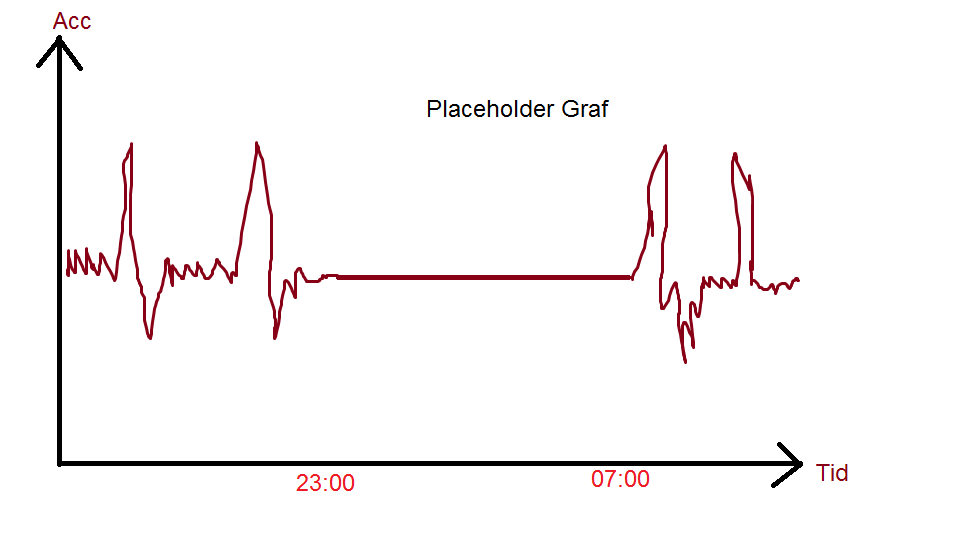
\includegraphics[scale=0.5]{acc-placeholder}
	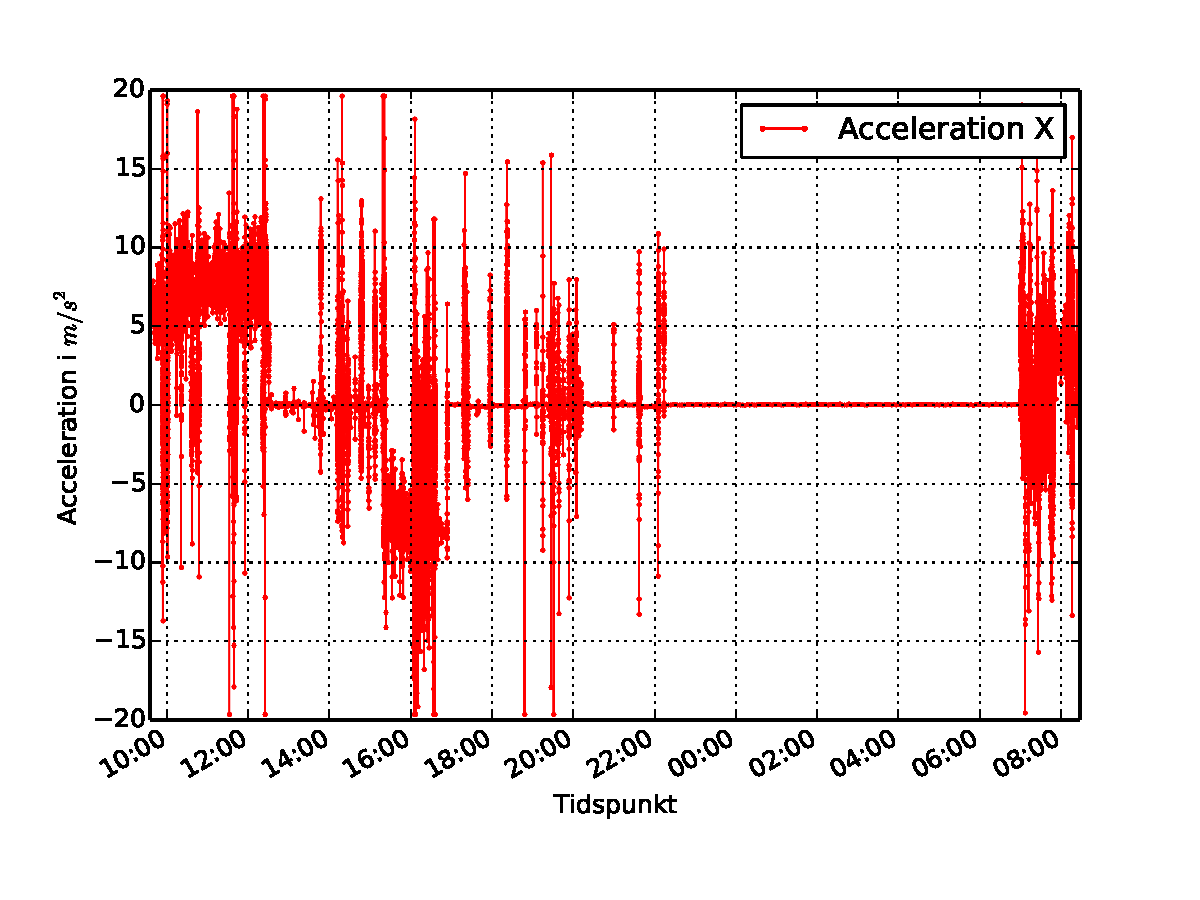
\includegraphics[scale=0.75]{acceleration-plot}
	\caption{Accelerationsplot, hvor der blev sovet fra ca. 22:00 til 07:00 næste dag.}\label{fig:accplot}
\end{figure}

Ses der på accelerometer data i \cref{fig:accplot} indikerer det tydeligt når telefonen har været i bevægelse.
Dette skyldes at i sensorens natur er den god til at registrere bevægelse, da accelerationer er nødvendige for at ændringer i hastighed kan finde sted.
Der kan ses at antagelsen om at når man går med sin telefon i lommen er man vågen svarer fint til accelerations plottet.
Dog kan man ved stilstand ikke vide sig sikker på om det er forbi man sover, eller blot fordi man har lagt sin mobil fra sig.
Ved stilstand i en længere periode kan det forsøges at estimere sandsynligheden for at denne stilstand er grundet at man sover, men derudover kan andre sensor inputs hjælpe til at klargøre denne tvivl, der ikke er begrænset til at man skal have telefonen i lommen.
Et eksempel på en sådan kilde er mikrofonen vi kan bruge til at måle maksamplitude, således at man ikke indsamler personfølsomme oplysninger.

\begin{figure}[h]
	\centering
	%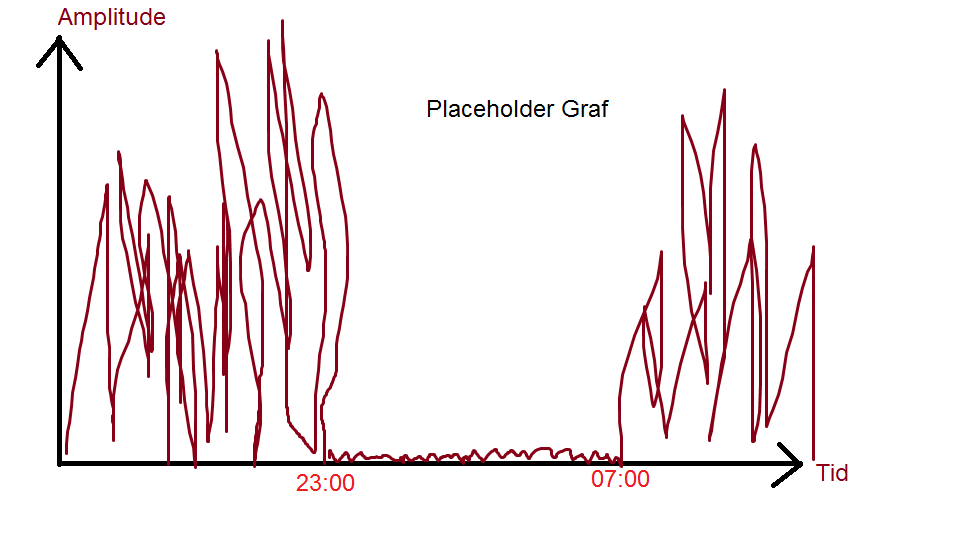
\includegraphics[scale=0.5]{ampl-placeholder}
	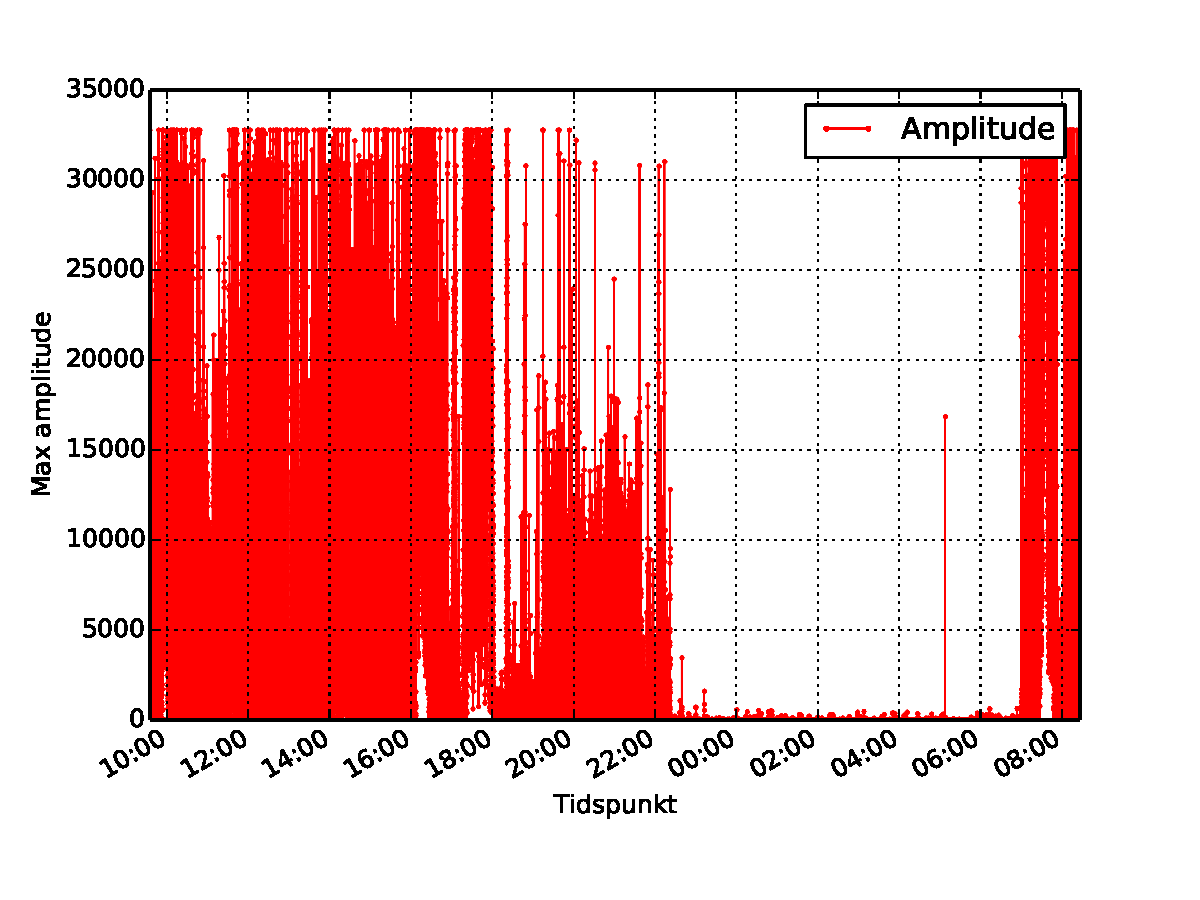
\includegraphics[scale=0.75]{amplitude-plot}
	\caption{Amplitudeplot, hvor der blev sovet fra ca. 22:00 til 07:00 næste dag.}\label{fig:amplplot}
\end{figure}

Idéen bag at bruge maksamplituden er at man larmer væsentligt mere når man er vågen end når man sover.
Dette passer fint med de loggede data plottet i \cref{fig:amplplot}.
Dog har denne antagelse også begrænsninger.
Eksempelvis kan det være at man er en stille person eller snorker meget.
Alligevel regner vi med at amplituden stadig kan bruges, da man så muligvis kunne finde et mønster når man snorker, og muligvis begiver sig hen i støjende områder når man er vågen. Derudover er det så et spørgsmål om hvor stor vægt man skal tillægge de enkelte sensorkilder og er noget der bør trænes til det enkelte individ for at opnå en model der passer til det enkelte individs personlighed.
Hvordan dette gøres bør overvejes, men som en start kan nogle fastsatte vægte bruges.

\subsection{Søvnestimerings model}
Ud fra observeret data etablerer vi nogle antagelser som vi går ud fra holder til fremtidigt data også.
Disse er at når man observerer en handling om det er acceleration eller amplitude, kan vi med stor sikkerhed sige at man ikke sover.
Modsat ved stilstand er sandsynligheden for at man sover afhængigt af længden af stilstand.
Dette får os til at lave en model der bygger på disse to antagelser.

Vi kan med andre ord sige følgende:
\begin{equation}
P(t,t_0) =
\begin{cases}
0	& t = t_0 \\
min(s(t-t_0),1) & \text{ellers}
\end{cases}
\end{equation}
hvor,
\begin{itemize}
	\item[$t$] Tiden for observeret data.
	\item[$t_0$] Sidste tid med bevægelse/lyd.
\end{itemize}
Hvis vi formulerer problemet på denne måde er det et spørgsmål om at ændre $t_0$ når der observeres et væsentligt udsving i ens data, der indikerer man er vågen.
Derudover vil $t-t_0$ så svare til længden af stilstand eksempelvis målt i timer.

Spørgsmålet går så på hvorledes $s(t-t_0)$ skal defineres.
Det skal være en funktion der repræsenterer hvor sikker man er på søvn ud fra længden af stilstand eksempelvis målt i timer.
En sådan funktion bør være lært ud fra ens empiri, så man kunne løse opgaven som et regressionsproblem.
Dette er et område der kan arbejdes videre med for at få en mere akkurat søvnestimeringsmetode og opfordres til at gøre med mere tid.

Dog for at få et udgangspunkt til diskussion af sådanne funktioner er der tre funktioner plottet i \cref{fig:trefunc}.
\begin{figure}[h]
	\centering
	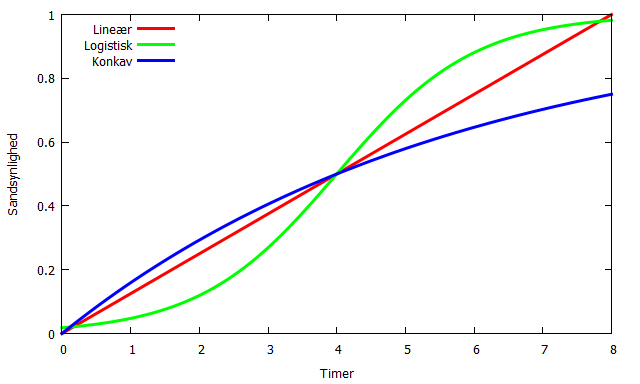
\includegraphics[scale=0.5]{graf-funktionseksempler}
	\caption{Tre funktioner til estimering af sandsynlighed for søvn}\label{fig:trefunc}
\end{figure}

\cref{fig:trefunc} viser tre forslag til funktioner for $s(t-t_0)$.
Disse er den røde lineære funktion, den blå konkave funktion og den grønne logistiske funktion.
Alle tre funktioner har til fælles at de er monotont voksende, hvilket passer med vores antagelse af jo længere der har været stilstand jo større sandsynlighed for at man sover.
Den lineære funktion bygger på antagelsen at sandsynligheden for at man sover er kongruent med stilstands længden, hvilket vi ikke ønsker da vi så tillægger for stor vægt til korte stilstandsperioder.
Af samme grund forkastes den konkave funktion også.

Til sidst har vi den logistiske funktion der fint beskriver hvordan at ved længere stilstandsperioden er der en forøget hældning i funktionen indtil vi nærmer os lange stilstandsperioder hvor ekstra tid ikke giver megen ekstra sandsynlighed for søvn men stadig lidt, dette kan ses da den logistiske funktion vi har plottet går asymptotisk mod 1, svarende til 100\% sikkerhed for søvn.
I realiteten kan vi aldrig være 100\% sikker på søvn ved lang stilstand, det kan være man har glemt mobilen hjemme mens man er på tur over en weekend, men hvis forudsætningen for at systemet fungerer er at man har mobilen i nærheden regnes den logistiske funktion som et godt redskab til et søvnestimat.

Definitionen af $s(t-t_0)$ hvor vi kalder $t-t_0$ for $t_{span}$ er dermed følgende:
\begin{equation}
	s(t_{span}) = \frac{L}{1+e^{k*(-t_{span} - t_{midpoint})}}
\end{equation} 
hvor,
\begin{itemize}
	\item[$t_{midpoint}$] er til hvilket stilstandslængde vi vil have sandsyngligheden for søvn til at være 50\%, dette kan eksempelvis være $4$ timer.
	\item[$k$] er stejlheden for kurven.
	\item[$L$] er kurvens maksimums værdi, hvilket for os eksempelvis kan være $1$ for 100\% sandsynlighed for søvn.
\end{itemize}

Der kan argumenteres for en lavere værdi for $L$ så man maks kan blive 90\% sikker, men er noget der bør overvejes med mere træningsdata.

Til sidst er der at orientere om hvordan vi afgør om der er stilstand, og dermed angiver en ny værdi for $t_0$, dette gøres i øjeblikket med en simpel metode der ser på de sidste 5 målinger og ser at afstanden mellem den observerede måling og de sidste fem målinger ikke overstiger et givet grænseværdi der estimeres ud fra træningsdataene, men i fremtiden bør der overvejes alternativer.

\subsection{Kombinering af modeller}
Det er tiltænkt at hver sensor kan have en tilknyttet søvnestimeringsmodel, hvilket i vores tilfælde er en søvnestimeringsmodel for accelerometer og mikrofon data.
Imidlertid kan det være en fordel at have en samlet model der kombinerer resultaterne fundet for de enkelte modeller.
En simpel metode at gøre dette på er v.h.a. et vægtet gennemsnit, hvilket er metode som \citet{6563918} også benytter.
Det vægtede gennemsnit kan udregnes på følgende måde:
\begin{equation}
	P_{kombineret}(t,t_0) = \sum_{i=1}^{n}{w_iP_i(t,t_0)}
\end{equation}
, hvor
\begin{itemize}
	\item[$P_{kombineret}(t,t_0)$] er den kombinerede sandsynlighed for søvn ved stilstand fra tiden $t_0$ til $t$.
	\item[$w_i$] er vægten som $P_i(t,t_0)$ skal tillægges.
	\item[$P_i(t,t_0)$] er sandsynligheden for søvn ved stilstand fra tiden $t_0$ til $t$ for sandlynlighedsmodellen $i$.
\end{itemize}
Dette er dog en forsimplet version af vores vægtede gennemsnit, i realiteten er der ikke data på samme tid eller i samme mængder for de enkelte søvnestimeringsmoduler.
Af samme grund ved mangel på en estimering til en given tid for et givent modul tages den seneste tid før denne.
Man kan forestille sig en lynlås hvor der skiftes mellem takkerne fra hver del, ligesom det gøres med estimeringerne for hvert modul.\als{SKAL HAVE EN BEDRE BESKRIVELSE}




\bibliographystyle{unsrtnat}
\bibliography{Bibliography}
\label{bib:mybiblio}

\appendix

\end{document}
